\documentclass[11pt]{jarticle}

\usepackage[dvipdfmx]{graphicx}

\setlength{\oddsidemargin}{-6.35mm}
\setlength{\textwidth}{171.9mm}

\begin{document}

\title{画像処理実験 第2回}
\author{09430509\\今田将也}
\date{2020年10月6日}
\maketitle

\section{(x,y)と(u,v)の位置に,ほぼ同じ物体が観測されていることを確認}
図\ref{kansoku}からほぼ同じ物体が同じ位置に観測されている
\begin{figure}[h]
    \centering
    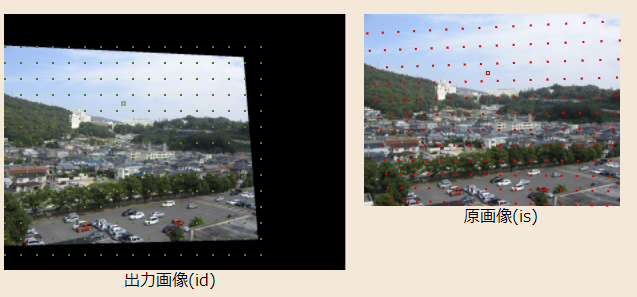
\includegraphics[scale=.5]{kansoku.png}
    \caption{出力画像と元画像}
    \label{kansoku}
\end{figure}

\section{射影変換 aの要素を変化させ画像の変化を確認}

\begin{verbatim}
    変更前の配列a
    a=[[ .866 , -.5  ,  160],
   [ .5   , .866 , -300],
   [-.001 , 0    ,    1]];

   変更後の配列a
   a=[[ .433 , -.5  ,  80],
   [ .5   , .433 , -150],
   [-.0001 , 0    ,    1]];
\end{verbatim}
\begin{figure}[h]
    \centering
    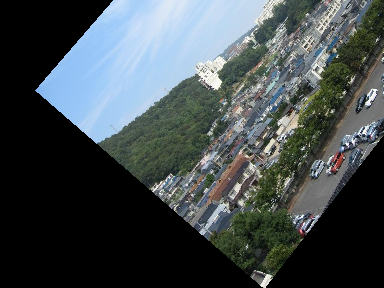
\includegraphics[scale=.5]{2kekka.png}
    \caption{配列変更後の出力画像}
\end{figure}

\section{C言語による実装例をもとに 上記と同様の処理を行う}
実装にあたり,ImageClear関数が定義されていなかったため,image.cにImageClear関数をまず定義した.
参考資料から,画像のすべての要素を黒で塗りつぶせば良いため,画像の画素数分ループ処理を行い,
全ての画素に黒の値である0を代入することで実装した.以下にそのソースを示す.
また結果は図\ref{cgengo}に示した.

\begin{verbatim}
    void ImageClear(Image *im){
    for(int y=0;y<im->H;y++){
        for(int x=0;x<im->W;x++){
            IElem(im,x,y,0) = 0;
            IElem(im,x,y,1) = 0;
            IElem(im,x,y,2) = 0;
        }
    }
}
\end{verbatim}
\begin{figure}[h]
    \centering
    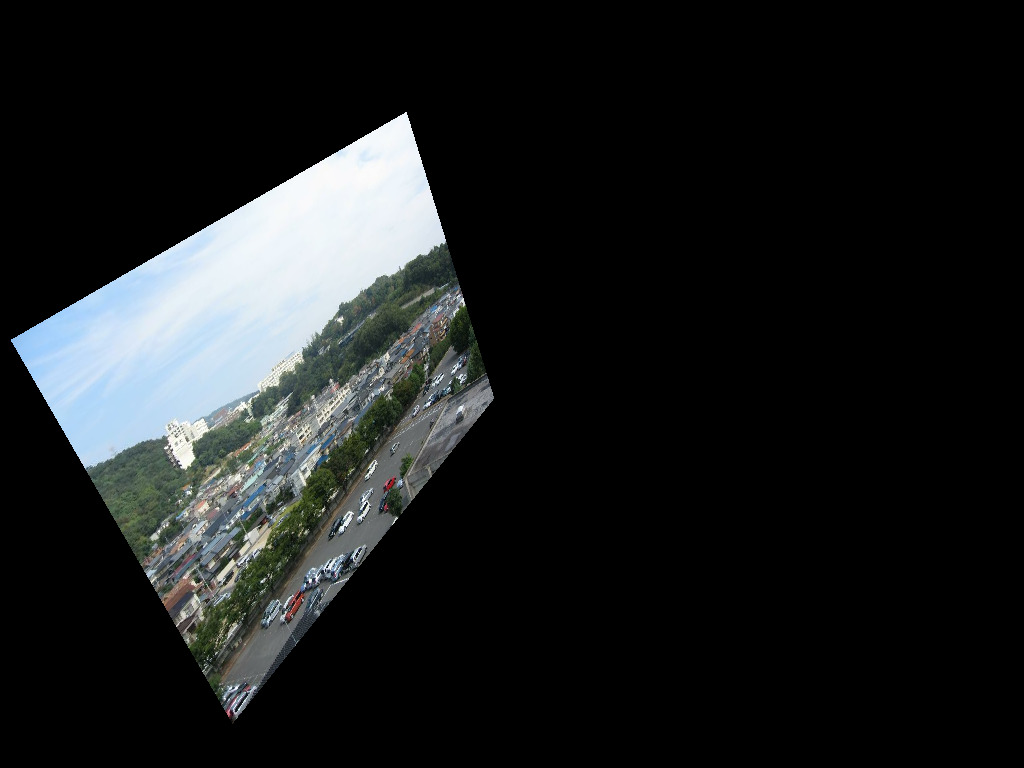
\includegraphics[scale=.15]{out1.jpg}
    \caption{C言語による処理結果}
    \label{cgengo}
\end{figure}

\section{m0d を適当な行列に変更しても,img1 と img0 の位置関係が保たれることを確認}
まず,図\ref{zurasumae}にm0d行列の変更前の画像を示す.
そして,次のように画像の全体の座標位置を右にずらすよう変更を加えたところ,図\ref{zurasu.png}のような
結果が得られた.
この結果から,img1とimg0の位置関係はm0dを適当な行列に変更しても保たれていることが確認できた.
\begin{verbatim}
    var m0d=[[ 2.667,0,-500 ],
         [ 0,2.667,-100 ],
         [ 0,0,1 ]];
\end{verbatim}
\begin{figure}[htbp]
    \begin{tabular}{cc}
        \begin{minipage}{0.5\hsize}
            \begin{center}
                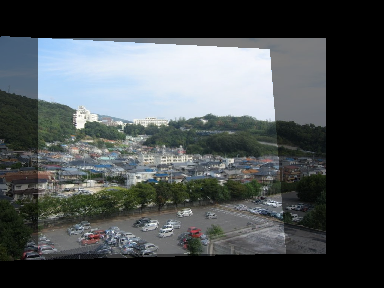
\includegraphics[scale=.5]{henkoumae.png}
                \caption{m0d行列変更前}
                \label{zurasumae}
            \end{center}
        \end{minipage}
        \begin{minipage}{0.5\hsize}
            \begin{center}
                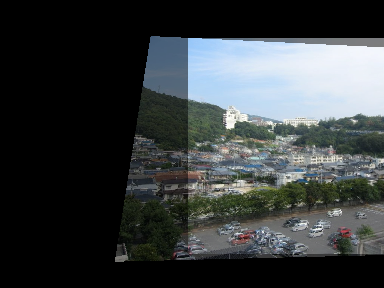
\includegraphics[scale=.5]{zurasu.png}
                \caption{m0d行列変更後}
                \label{zurasu.png}
            \end{center}
        \end{minipage}
    \end{tabular}
\end{figure}

\section{行列 m10 を修正し,ずれのない合成画像を作成することを試みる}
いくつかの行列を修正し,試みたがうまくずれをなくすことができなかった.

\section{m10 を算出し,合成に用いなさい}
実験のページに記載されているページの特徴点を動かすことで正しいm10を算出し,合成に用いた.
合成をしたい元画像の両方で特徴点が正確に同じ物体を指すようにするということを行い算出をした.
以下が算出した配列である.
なお,図\ref{sansyutu}が合成後の画像である.左下の部分をみると多少ブレが見られるものの多くの部分で
ブレがなくなっているためこの配列を回答とした.
\begin{verbatim}
    0.930421    0.018946    118.490952
    -0.043542   0.976597    22.193656
    -0.000097   0.000002    1.000000 
\end{verbatim}
\begin{figure}[h]
    \centering
    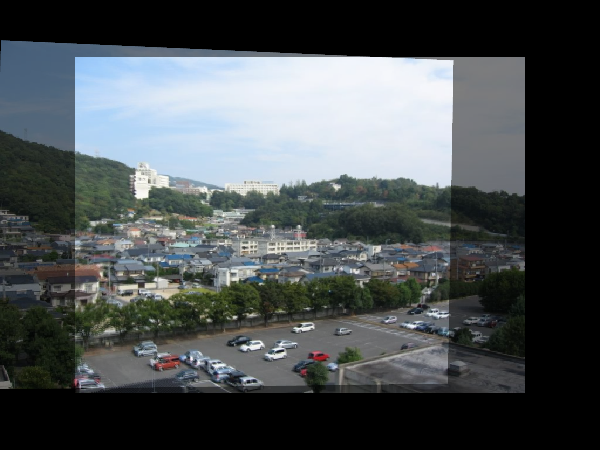
\includegraphics[scale=.5]{sansyutu.png}
    \caption{m10を修正した後の合成画像}
    \label{sansyutu}
\end{figure}

\section{3x3 行列の積を計算する関数 mult33 を実装し,m1d = m10 ˙ m0d を計算し,画像を合成}
3x3行列は,左の行列1行目の各要素を右側の行列1列目の各要素にかけて,それら3つの項を足しあわせ,1行1列要素
とする.左の行列1行目の各要素を右側の行列2列目の各要素にかけて・・・という手順を繰り返していき,3行3列要素目までを計算すればよい.

その実装としては,2重ループを用いて行った.左側は右側の3つ分が終わると次の行に進み,また,掛け合わす場所は定義より決まっているため,
以下のソースコードのようにした.
\begin{verbatim}
    void mult33(double d[3][3],double a[3][3],double b[3][3]){
    for(int i=0;i<3;i++){
        for(int j=0;j<3;j++){
            d[i][j] = a[i][0]*b[0][j] + a[i][1]*b[1][j] + a[i][2]*b[2][j]; 
        }
    }
}
\end{verbatim}
そして,これをpano0.cのmain関数にて使用したのが以下である.
ImageImageProjectionAlpha は,行列 m0d を使って im (0.jpg) を id に書き込む.m0dは結果を出力画像の中心寄りに表示するための平行移動
(右に100,下に100)を行う射影変換である.
行列 m1d を使った ImageImageProjectionAlpha は,id に im (1.jpg) を書き込む.m10 は img1 と img0 の関係を表し,m0d は img0 と 出力画像の関係を表す.
img1 と出力画像の関係は m10 と m0d の積で表される.このときに
パノラマ合成を行う必要があり,m10に,先程求めた算出後の配列を使用.また,m1dはm10とm0dの積で表されるため,
mult33を使い,積を計算した.パノラマ合成後の結果画像は図\ref{panorama}に示した.

\begin{verbatim}
    double m0d[][3]={
      1,0,-100,
      0,1,-100,
      0,0,1
    };
    im=ImageRead("0.jpg");
    ImageImageProjectionAlpha(id,im,m0d,.5);
    double m10[][3]={
      0.930421,   0.018946,   118.490952,
      -0.043542,  0.976597,   22.193656,
      -0.000097,  0.000002,   1.000000 
    }, m1d[3][3];
    mult33(m1d,m10,m0d);
\end{verbatim}

\begin{figure}[h]
    \centering
    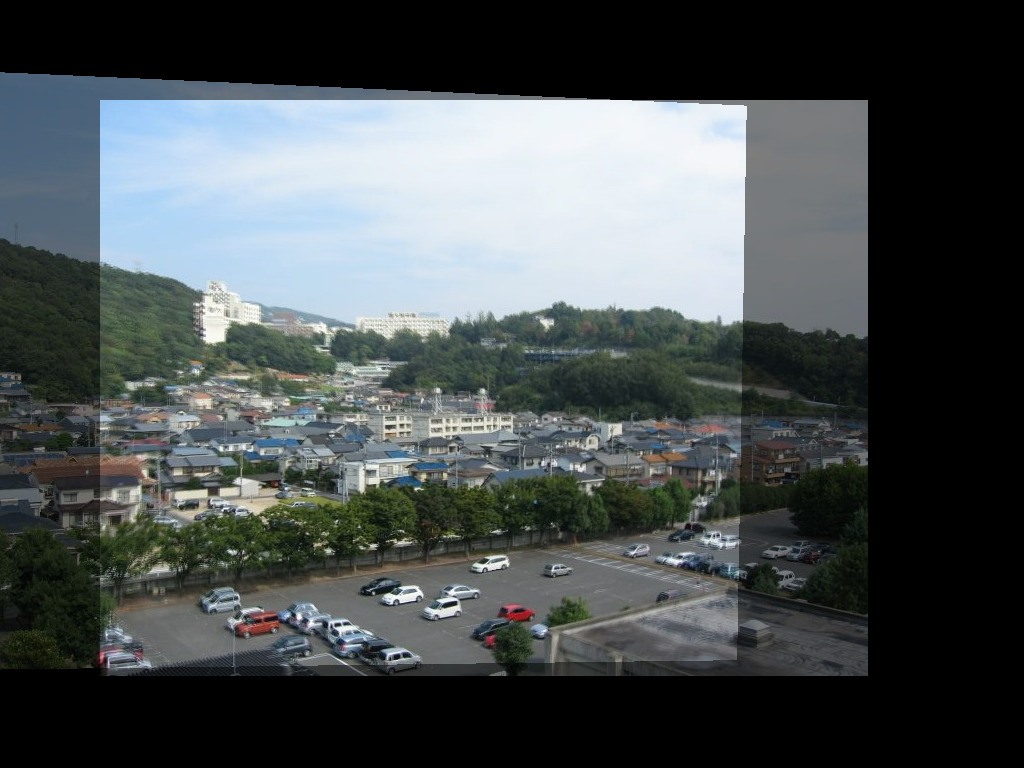
\includegraphics[scale=.3]{panorama.png}
    \caption{C言語でのパノラマ合成の結果画像}
    \label{panorama}
\end{figure}

\section{「原画像の座標(u,v)を出力画像の座標(x,y)に変換する行列」を A とすると,上記の実装で用いている a は A の逆行列である.}
これを確認するために,
    $ \left(
        \begin{array}{rrr}
        2 & 0 & 0 \\
        0 & 2 & 0 \\
        0 & 0 & 1
        \end{array}
    \right) $
の,逆行列
$ \left(
    \begin{array}{rrr}
    0.5 & 0 & 0 \\
    0 & 0.5 & 0 \\
    0 & 0 & 1
    \end{array}
\right) $
をかけたときに2倍になるかどうかを見る.

homography.cの配列aを先程の逆行列のように変え,実行すると図\ref{kakudai}のようになった.
\begin{figure}[h]
    \centering
    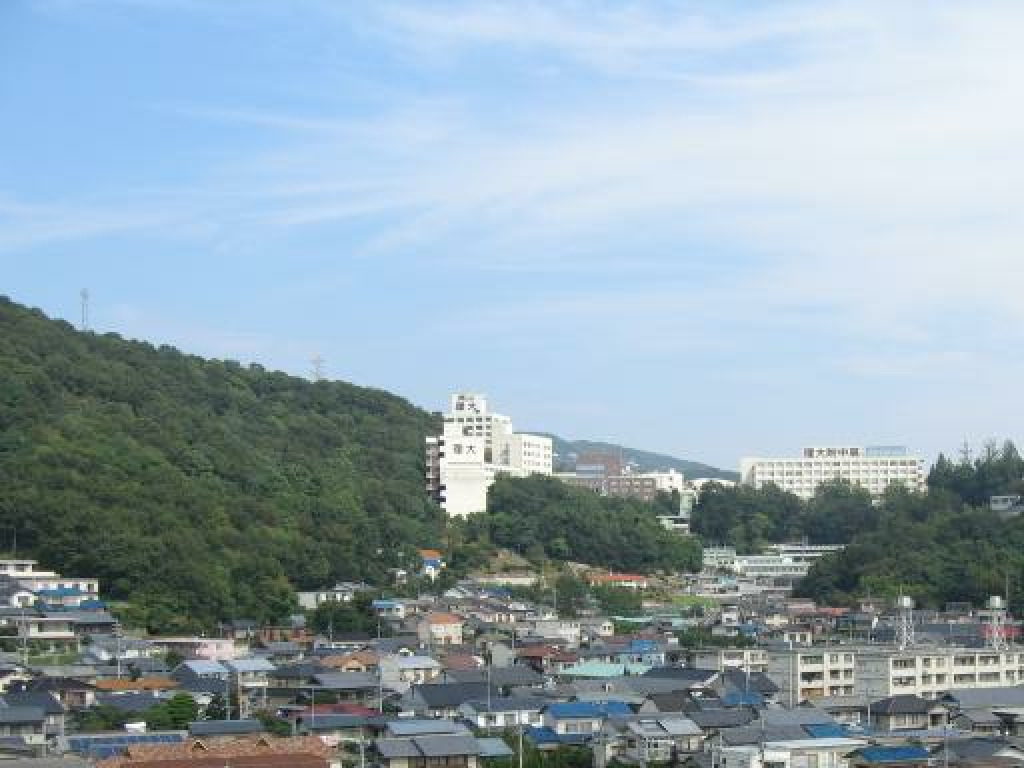
\includegraphics[scale=.2]{kakudai.jpg}
    \caption{結果}
    \label{kakudai}
\end{figure}

きちんと拡大されていたことが確認できた.
\section{感想}
パノラマ画像の生成ができた.ヘッダーファイルからの読み込み方法や,行列の計算式など
基本的な実装も危うかったのでちょっと大変でしたがなんとかできました.

最後の確認の問題が難しかったです.

\end{document}
